\documentclass[a4paper,12pt]{report}
\usepackage[toc,page]{appendix}
\usepackage{amsmath}
\usepackage{float}
\usepackage{graphicx}
\usepackage{subfig}
\usepackage{amssymb}
\usepackage{geometry}
\usepackage{mathtools}
\usepackage{pgfplots}
\pgfmathdeclarefunction{gauss}{2}{%
  \pgfmathparse{1/(#2*sqrt(2*pi))*exp(-((x-#1)^2)/(2*#2^2))}%
}
\usepackage{setspace}
 \geometry{
 a4paper,
 total={170mm,257mm},
 left=20mm,
 top=20mm,
 }
\usepackage{tikz}
\usepackage{pgfplots}
\usetikzlibrary{shapes, arrows.meta, decorations.pathreplacing, positioning, petri, fit, calc}
\tikzstyle{startstop} = [rectangle, rounded corners, minimum width=2cm, minimum height=0.5cm,text centered, text width=3cm, draw=black, fill=gray!30]
\tikzstyle{process} = [rectangle, minimum width=2cm, minimum height=0.5cm, text centered, text width=3cm, draw=black, fill=blue!30]
\tikzstyle{detail} = [rectangle, minimum width=7cm, minimum height=0.5cm, text justified, text width=6.5cm, draw=black, fill=white!30]
\tikzstyle{smalldetail} = [rectangle, minimum width=3.5cm, minimum height=0.5cm, text justified, text width=3cm, draw=white, fill=white!30]
\tikzstyle{decision} = [rectangle, minimum width=3cm, minimum height=1cm, text centered, draw=black, fill=green!30]

\usepackage[utf8]{inputenc}

% Default fixed font does not support bold face
\DeclareFixedFont{\ttb}{T1}{txtt}{bx}{n}{10} % for bold
\DeclareFixedFont{\ttm}{T1}{txtt}{m}{n}{10}  % for normal

% Custom colors
\usepackage{color}
\definecolor{deepblue}{rgb}{0,0,0.5}
\definecolor{deepred}{rgb}{0.6,0,0}
\definecolor{deepgreen}{rgb}{0,0.5,0}

\usepackage{listings}

% Python style for highlighting
\newcommand\pythonstyle{\lstset{
language=Python,
basicstyle=\ttm,
otherkeywords={self},             % Add keywords here
keywordstyle=\ttb\color{deepblue},
emph={MyClass,__init__},          % Custom highlighting
emphstyle=\ttb\color{deepred},    % Custom highlighting style
stringstyle=\color{deepgreen},
frame=tb,                         % Any extra options here
showstringspaces=false            % 
}}


% Python environment
\lstnewenvironment{python}[1][]
{
\pythonstyle
\lstset{#1}
}
{}

% Python for external files
\newcommand\pythonexternal[2][]{{
\pythonstyle
\lstinputlisting[#1]{#2}}}

% Python for inline
\newcommand\pythoninline[1]{{\pythonstyle\lstinline!#1!}}


\begin{document}
\tableofcontents

\title{Machine Learning}
\maketitle
\part{Week 1 and 2}
\section{Introduction / Definition }
\subsection{What is Machine Learning?}
\textbf{Machine Learning}: algorithms for \textbf{inferring} unknowns from knowns.
\\ \\

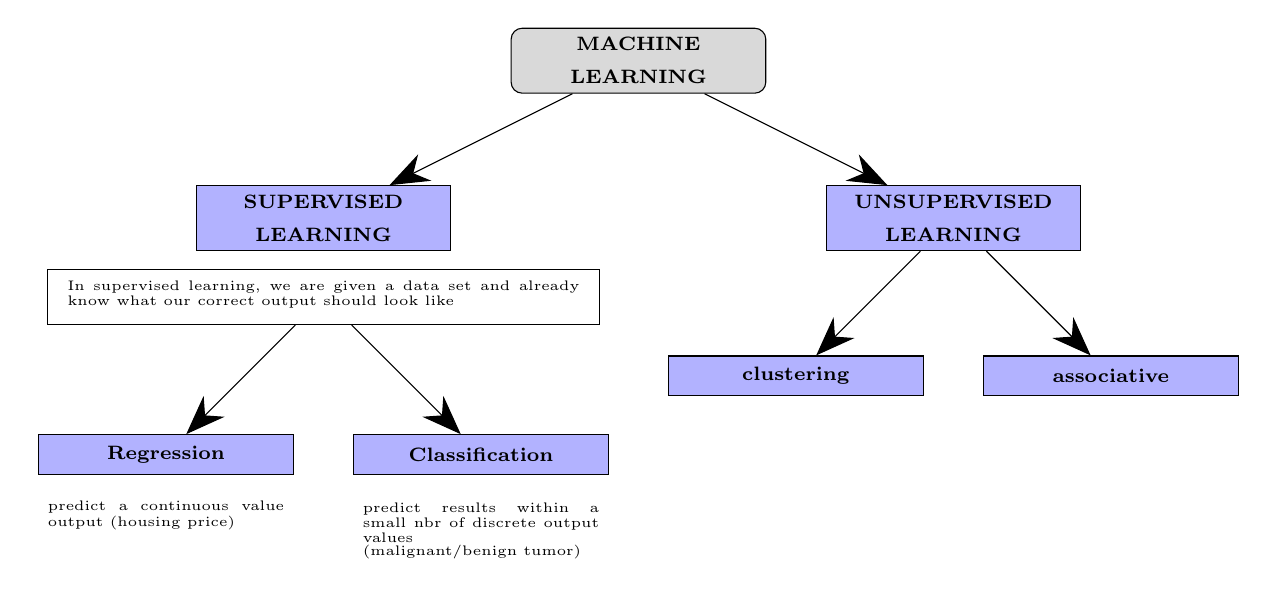
\begin{tikzpicture}[node distance=4cm]
\node (start) [startstop] {{\scriptsize \textbf{MACHINE LEARNING}}};
\node (pro2a) [process, below of=start, xshift=-4cm, yshift=2cm] {{\scriptsize \textbf{SUPERVISED LEARNING}}};
\node (det1a) [detail, below of=pro2a, xshift=0cm, yshift=3cm] {\begin{spacing}{0.2}{\tiny In supervised learning, we are given a data set and already know what our correct output should look like}\end{spacing}};
\node (pro2b) [process, below of=start, xshift=4cm, yshift=2cm] {{\scriptsize \textbf{UNSUPERVISED LEARNING}}};
\node (pro2d) [process, below of=det1a, xshift=-2cm, yshift=2cm] {{\scriptsize \textbf{Regression}}};
\node (det1b) [smalldetail, below of=pro2d, xshift=0cm, yshift=3.2cm] {\begin{spacing}{0.2}{\tiny predict a continuous value output (housing price)}\end{spacing}};
\node (pro2e) [process, below of=det1a, xshift=2cm, yshift=2cm] {{\scriptsize \textbf{Classification}}};
\node (det1c) [smalldetail, below of=pro2e, xshift=0cm, yshift=3cm] {\begin{spacing}{0.2}{\tiny predict results within a small nbr of discrete output values \\(malignant/benign tumor)}\end{spacing}};
\node (pro3a) [process, below of=pro2b, xshift=-2cm, yshift=2cm] {{\scriptsize \textbf{clustering}}};
\node (pro3b) [process, below of=pro2b, xshift=2cm, yshift=2cm] {{\scriptsize \textbf{associative }}};

\draw[-{Stealth[length=5mm]}] (start) -- (pro2a);
\draw[-{Stealth[length=5mm]}] (start) -- (pro2b);
\draw[-{Stealth[length=5mm]}] (det1a) -- (pro2d);
\draw[-{Stealth[length=5mm]}] (det1a) -- (pro2e);
\draw[-{Stealth[length=5mm]}] (pro2b) -- (pro3a);
\draw[-{Stealth[length=5mm]}] (pro2b) -- (pro3b);
\end{tikzpicture}

\subsection{Supervised Learning}
\begin{itemize}  
\item \textbf{a regression problem: predict housing price }
\begin{figure}[H]
\centering
        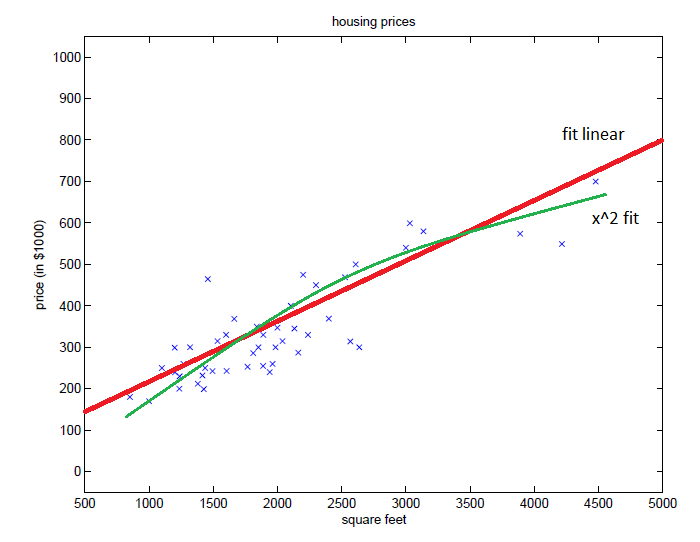
\includegraphics[totalheight=4 cm]{housingData.png}
						\caption{
								\label{housingData} The right answer in this example is the price corresponding to the house size. }
\end{figure}

\item \textbf{a classification problem: predict if tumor is malignant or benign. }
\begin{figure}[H]
\centering
        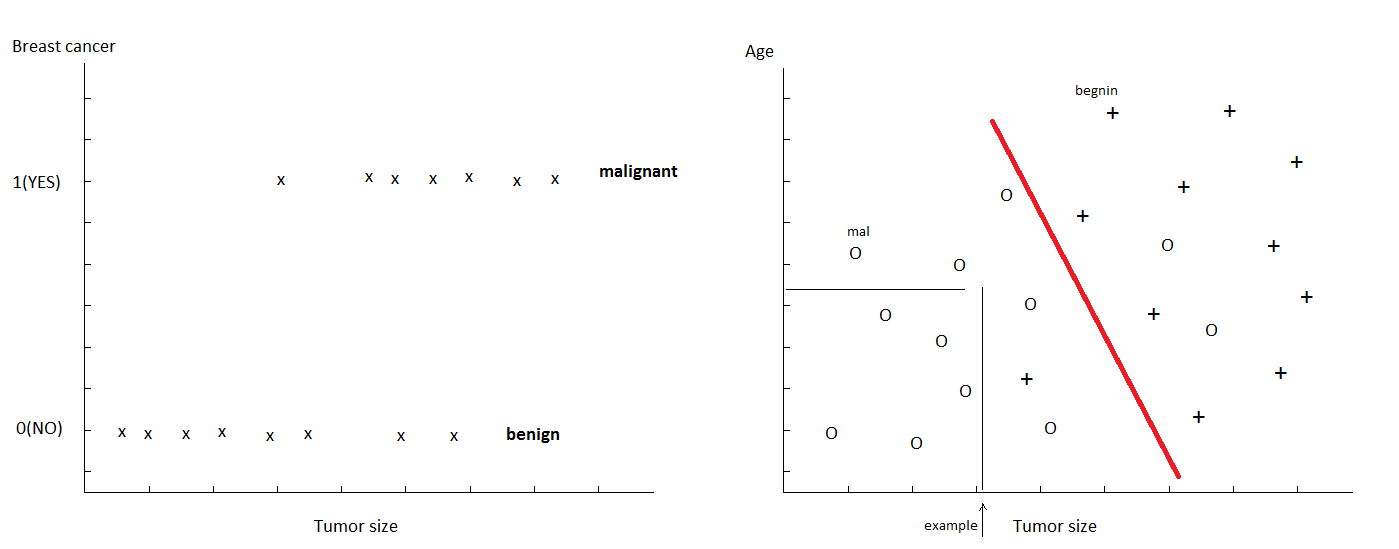
\includegraphics[totalheight=4 cm]{breastCancer.png}
						\caption{
								\label{breastcancer} In classification problems, one can have more than 2 values for the output: for example may be 3 types of cancer (0=benign, 1=malignant, 2=type2, 3=type3). The graph on the right shows an alternative way of plotting  the data when using several features / attributes. The learning algorithm may decide to separate the malign and benign with a straight line, hence the example of with shown age and tumor size would have a high probability to be a malign tumor }
\end{figure}

\end{itemize}

\subsection{Supervised vs. Unsupervised Learning}
\begin{itemize}
\item in \textbf{supervised} learning, each \textbf{example is labeled}.
	\begin{itemize}
		\item regression
		\item classification
	\end{itemize}
\item in \textbf{unsupervised learning}, there is \textbf{no label}: the algorithm might look for some structures in the data, and might separate the data in to 2 clusters (clustering algorithm). Examples where unsupervised Learning algorithm is used: organize computing clusters, social network analysis, market segmentations. 
\begin{itemize}
	\item clustering
	\item density estimation
	\item Dimensionality reduction
\end{itemize}
\begin{figure}[H]
\centering
        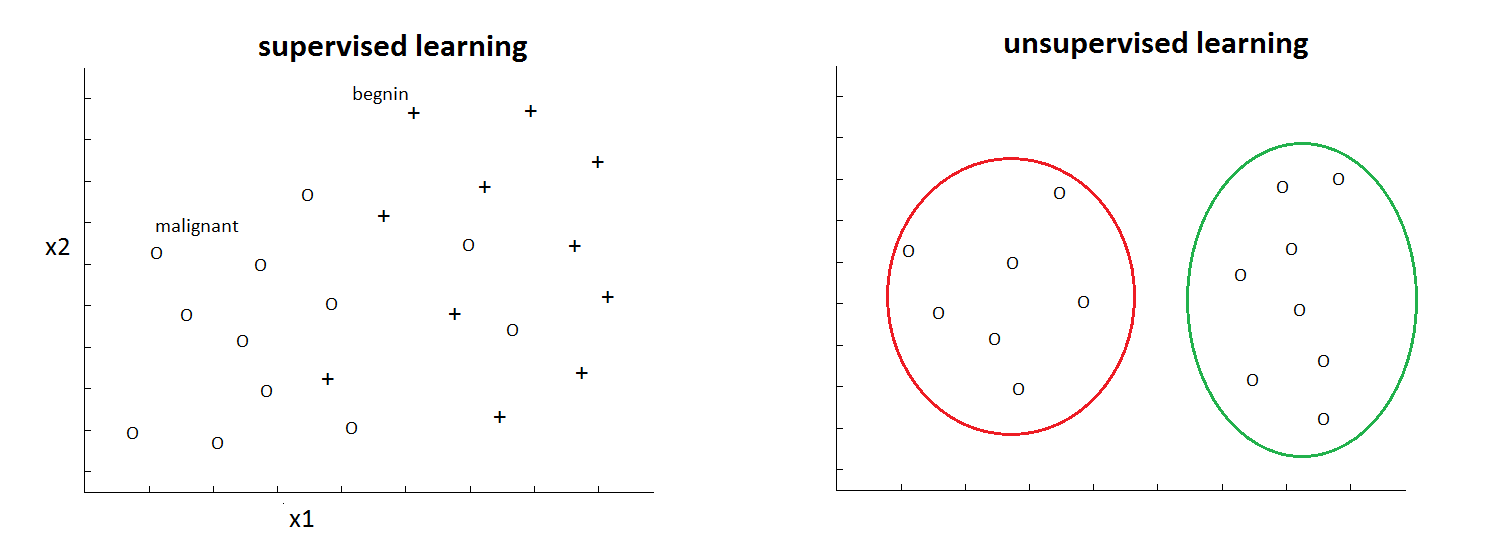
\includegraphics[totalheight=4 cm]{supervisedVSunsuper.png}
						\caption{
								\label{superVSunsuper} Illustration of supervised and unsupervised learning}
\end{figure}
\end{itemize}
\begin{figure}
\centering
\begin{tikzpicture}[baseline]
\begin{axis}[
no markers, domain=-10:10, samples=100,
axis y line=center,
axis x line=middle,
grid=both,
xmax=10,xmin=-10,
ymin=-0.1,ymax=1,
xlabel=$x$,ylabel=$y$,
xtick={-10,-5,0,510},
ytick={-1,-0.5,0,0.5,1},
width=10cm,
anchor=center,
]
\addplot {{1.5*gauss(1,1) + 1*gauss(-2,1) + 0.6*gauss(6,1)}} ;
\end{axis}
\end{tikzpicture}
\caption{This is an example of density estimation. The $x$ axis has a distribution of data point centered at -2, 1 and 6}
\end{figure}

There are some variations:
\begin{itemize}
\item Semi-supervised learning: mix of labeled and unlabeled dataset
\item Active learning
\item Decision Theory
\item Reinforced learning
\end{itemize}
\section{Generative vs. Discriminative models}
\subsection{Discriminative models}
Discriminative approach would model the probability $p(y|x)$ i.e probability of $y$ given x.

\subsection{Generative model}
Generative approach models the joint probability distribution i.e $p(x, y)$ (probability of $x$ and $y$ ).
\newline
\begin{align}
p(x,y) = f(x|y) p(y)
\end{align}
where $f(x|y)$ is the density of $x$ given $y$, and $p(y)$ ist the probability of $y$.
\section{Supervised Learning: Linear regression with 1 variable/feature (aka univariable linear regression)}
\textbf{The Goal is to predict a unique output from a single input value.}

\begin{enumerate}
\item The hypothesis function $h_{\theta}(x)$ (or $h_{\theta}$):
\begin{equation}
		\label{hypo} h_{\theta} (x) = \theta_0 + \theta_1 x,
\end{equation}
where $\theta$'s are the parameters

\item The cost function (or squared error function or Mean Squared Error): measure the accuracy of our hypothesis function.
\begin{equation}
		\label{errfn} J(\theta_0, \theta_1) = \frac{1}{2m} \sum _{i=1} ^{m} \left(h_{\theta}(x^{(i)}) -y^{(i)} \right)^2,
\end{equation}
where $\left(h_{\theta}(x^{(i)}) -y^{(i)} \right)^2$ is the difference between the predicted value and the actual value, and $m$ is the size of the training set (data set). $x^{(i)}$ and $y^{(i)}$ are values of examples in the given training set.

\item Gradient Descent method: to automatically improve hypothesis function.\\
\noindent\rule{18cm}{0.4pt}\\
\textit{Repeat until convergence} \{
\begin{align*}
		\label{graddesc} \theta_j := \theta_j - \alpha \frac{\partial}{\partial \theta_j} J(\theta_0, \theta_1)
\end{align*}
simultaneous update of all $\theta$'s: $j=0$ and $j=1$. \\
\} \\
\noindent\rule{18cm}{0.4pt}\\

where $\alpha$ is called the learning rate. \\
The goal is to minimize the cost function i.e get $\theta_0$ and $\theta_1$ value for which the difference between predicted and real value is the smallest.\\
\end{enumerate}
\textbf{Gradient descent for linear regression:} \\
Using definition of $h_{\theta}$ and $J(\theta_0, \theta_1)$: \\
\noindent\rule{18cm}{0.4pt}\\
Repeat until convergence \{
\begin{align*}
		 \theta_0 & := \theta_0 - \alpha \frac{1}{m} \sum _{i=1} ^m \left(h_{\theta}(x^{(i)}) - y^{(i)} \right) \\
		 \theta_1 &:= \theta_1 - \alpha \frac{1}{m} \sum _{i=1} ^m \left(h_{\theta}(x^{(i)}) - y^{(i)} \right) \times x^{(i)} \\
\end{align*}
simultaneous update for $\theta_0$ and $\theta_1$ \\
\} \\
\noindent\rule{18cm}{0.4pt}


\subsection{Application to the house pricing example}
Provided training set: \\ \\
{
\centering
\begin{tabular}{ p{3cm} |p{3cm}||p{3cm}||  }
\hline
\hline
 & size in ft$^2$ ($x$)& Price \$\$ ($y$)\\
 \hline
 ($x$,$y$) $\rightarrow$ & 2104  \ $\leftarrow x^{(1)}$   & 460 \ $\leftarrow y^{(1)}$\\
 &   1600 \ $\leftarrow x^{(2)}$   & 330 \ $\leftarrow y^{(2)}$\\
 &   2400  \ $\leftarrow x^{(3)}$  & 369 \ $\leftarrow y^{(3)}$\\
 &   1416  \ $\leftarrow x^{(4)}$  & 232 \ $\leftarrow y^{(4)}$\\
 &   3000  \ $\leftarrow x^{(5)}$  & 540 \ $\leftarrow y^{(5)}$\\
 &. &.\\
 &. &.\\
 & .... \ $\leftarrow x^{(m)}$ & ... \ $\leftarrow y^{(m)}$\\
\end{tabular}
}
\begin{itemize}
\item $x$ = input variables / features
\item $m$ is the total number of training examples
\item $y$ = output variable / target variable
\item ($x,y$) = one training example
\item ($x^{(i)},y^{(i)}$) = $i^{\mathrm{th}}$ training example
\end{itemize}

\begin{itemize}
\item Picture of the process: \\
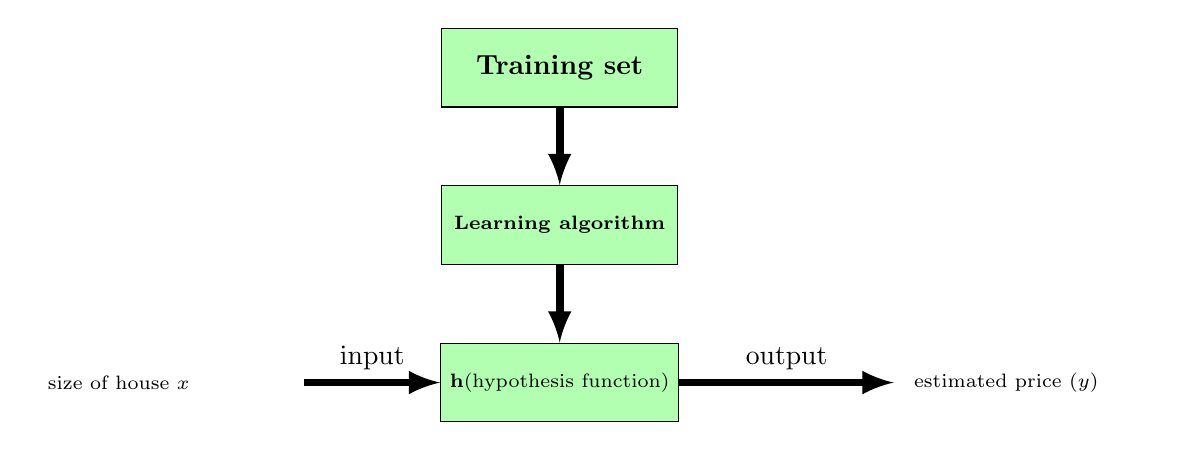
\begin{tikzpicture}[node distance=4cm]
\node (start1) [decision] {\textbf{Training set}};
\node (dec1a) [decision, below of=start1, xshift=0cm, yshift=2cm] {{\scriptsize \textbf{Learning algorithm}}};
\node (dec1b) [decision, below of=dec1a, xshift=0cm, yshift=2cm] {{\scriptsize \textbf{h} \\(hypothesis function)}};
\node (det1a) [smalldetail, below of=dec1a, xshift=-5cm, yshift=2cm] {{\scriptsize size of house $x$}};
\node (det1b) [smalldetail, below of=dec1a, xshift=6cm, yshift=2cm] {{\scriptsize estimated price ($y$)}};
\draw[-latex,line width=1mm] (start1) -- (dec1a);
\draw[-latex,line width=1mm] (dec1a) -- (dec1b);
\draw[-latex,line width=1mm] (det1a) -- node[anchor=south]{input} (dec1b);
\draw[-latex,line width=1mm] (dec1b) -- node[anchor=south]{output} (det1b);
\end{tikzpicture}
\\
In this example, we take a linear representation of $h$ (i.e linear regression with one variable or \textbf{univariante linear regression}):
$h_{\theta} (x) = \theta_0 + \theta_1 x$

\item Result
\begin{figure}[H]
\centering
        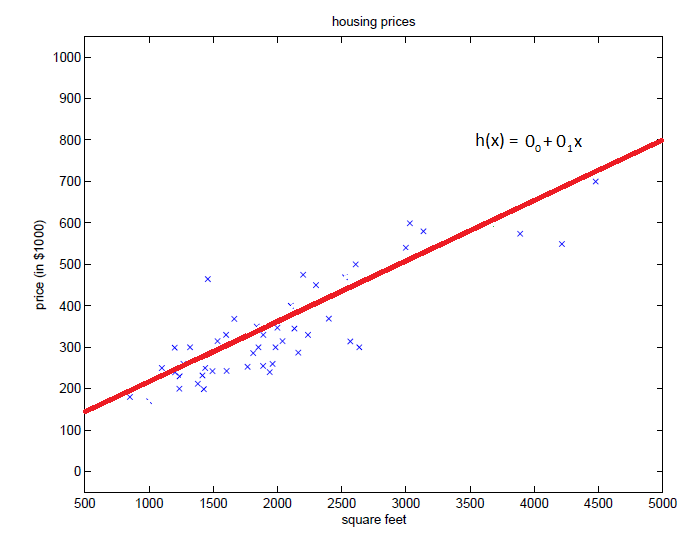
\includegraphics[totalheight=4 cm]{housinglinReg.png}
						\caption{Result: the red line is the best fit from Gradient descent.
								\label{fig2} }
\end{figure}
\end{itemize}


\section{Multiple features}
\subsection{Hypothesis function for $n$ features}
For 1 feature, the hypothesis was:
\begin{align*}
		\begin{split}
				h_{\theta}(x)  & = \theta_0 + \theta x_1 \\
				& = \theta_0 x_0 + \theta x_1  \\
		\end{split}
\end {align*}
where $x_0 = 1$ by convention.  \\ \\

Let's now consider the case of 4 features: \\
{
\centering
\begin{tabular}{ p{1cm} | p{3cm} | p{3cm} | p{3cm} | p{3cm} ||p{2cm}||  }
\hline
\hline
 $x_0$ & size in ft$^2$ ($x_1$)& Nbr of Bdr ($x_2)$ & Nbr of floors ($x_3)$ & Age home ($x_4)$  & Price \$\$ ($y$)\\
 \hline
 1 & 2104   & 5 & 1 & 45 & 460 \\
 1 & 1416   & 3 & 2 & 40 & 232 \\
 1 & 1534   & 3 & 2 & 30 & 315 \\
 1 & 852    & 2 & 1 & 36 & 178 \\
 1 & . &. & & & \\
 . &. &. & &  & \\
1 & ($x_1 ^{(m)}$) & ($x_2 ^{(m)}$) & ($x_3 ^{(m)}$) & ($x_4 ^{(m)}$) & ($y^{(m)}$)\\
\end{tabular}
}

\begin{itemize}
\item $n$ is the number of features (4)
\item $x_j ^{(i)} = $ value of features $j$ in $i^{\mathrm{th}}$ training example
\item $x^{(2)} = \left[ \begin{smallmatrix} 1 \\ 1416 \\ 3 \\ 2 \\ 40 \end{smallmatrix} \right] $
is a vector matrix of size 4 ($\mathbb{R} ^ {4 \times 1}$), showing the feature values of training example 2.
\end{itemize}

With $x_0=1$, the hypothesis for $n$ features can take the general form (multivariate linear regression):		

\begin{equation}
	\begin{split}
			\label{h_multi} 
			    h_{\theta}(x) & = \theta_0 x_0 + \theta_1 x_1 + \theta_2 x_2 + ...... \theta_n x_n \\
					              & = \sum _{j=0} ^{n} \theta_j x_j \\
												& = \theta ^{\mathrm{T}} X   \mathrm{vectorized \ form}
		\end{split}
\end{equation}
where:
\begin{itemize}
\item 
$X = \left[ \begin{smallmatrix} 1 & 2104   & 5 & 1 & 45\\
 1 & 1416   & 3 & 2 & 40\\
 1 & 1534   & 3 & 2 & 30\\
 1 & 852    & 2 & 1 & 36\\
 1 & . &. & . & . \\
 . &. &. & . & . \\
1 & (x_1 ^{(m)}) & (x_2 ^{(m)}) & (x_3 ^{(m)}) & (x_4 ^{(m)})\\
 \end{smallmatrix} \right]$   $\in \mathbb{R} ^ {m \times (n+1)}$
\item $\theta = \left[ \begin{smallmatrix} \theta_0 \\ \theta_1 \\ . \\ . \\ . \\ \theta_n \end{smallmatrix} \right]$   $\in \mathbb{R} ^ {n \times 1}$
\end{itemize}

\subsection{ The Cost function $J(\theta)$}
\begin{align*}
	\begin{split}
				J(\theta_0, \theta_1, \theta_2,...., \theta_n) & = J(\theta) \\
				                                               & = \frac{1}{2} \sum _{i=1} ^m \left( h_{\theta}(x^{(i)}) - y^{(i)} \right)^2
	\end{split}
\end {align*}

\subsection{Gradient descent algorithm}
\noindent\rule{10cm}{0.4pt} 
\\ \textit{Repeat until convergence} \{
\begin{align*}
\theta_j  := \theta_j - \alpha \frac{\partial}{\partial \theta_j} J(\theta)\\
\end{align*}
(update all $\theta_j$ simultaneously: $j = 0$ to $n$).
\} \\
\noindent\rule{10cm}{0.4pt}

This is called "`batch Gradient Descent"': each step of gradient descent uses \textbf{all} the training examples (1 through $m$). This method is not appropriate (too heavy) when dealing with very high number of features (1+ million). An alternative is "`\textbf{Stochastic Gradient Descent}"':
\noindent\rule{10cm}{0.4pt} 
\\ \textit{Repeat until convergence} \{
for $i=1$ to $m$, \{
\begin{align*}
\theta_j  := \theta_j - \alpha (h_{\theta}(x^{(i)}) - y^{(i)} ) x_j ^{(i)}
\end{align*}
(for every $j$).
\} \\
\} \\
\noindent\rule{10cm}{0.4pt}
\\
In this algorithm, we repeatedly run through the training set, and each time we encounter a training example, we update the parameters according to the gradient of the error with respect to that single training example only. Often stochastic gradient descent gets $\theta$ "`close"' to the minimum much faster than batch gradient descent (note however that it may never converge to the minimum, and $\theta$ will keep oscillating around the minimum of $J(\theta)$).  
\noindent\rule{10cm}{0.4pt} 
\\ \textit{Repeat until convergence} \{
\begin{align*}
\theta_j  := \theta_j - \alpha \frac{\partial}{\partial \theta_j} J(\theta)\\
\end{align*}
(update all $\theta_j$ simultaneously: $j = 0$ to $n$).
\} \\
\noindent\rule{10cm}{0.4pt}

\section{Gradient descent in practice}
In practice, we stop the iteration when $\frac{\partial J}{\partial \theta} < \epsilon$, where $\epsilon$ is a tolerance set by the user.
\subsection{Feature scaling: how to converge faster}
Place all the features at same scale:
\begin{enumerate}
\item method 1: features range $\Rightarrow$ $-1 \leq x_j \geq 1$ \\
eg: $x_1 = $size (0-2000) and $x_2=$ Nbr of bdrs (1-5).
Use $x_1=($size / 2000)  $x_2=($bdr / 5)
\item method 2: mean normalization $\Rightarrow$ $-0.5 \leq x_j \geq 0.5$ \\
Replace  $x_j$ by $(x_j - \mu_j)/s_j$ where $\mu_j$ is the mean of $x_j ^i$ for all $i$'s (i.e over all training examples), and $s_j$ is the range, either (max-min) or stdev. 
\end{enumerate}

\subsection{Learning rate $\alpha$: how to converge faster}
\begin{figure}[H]
\centering
        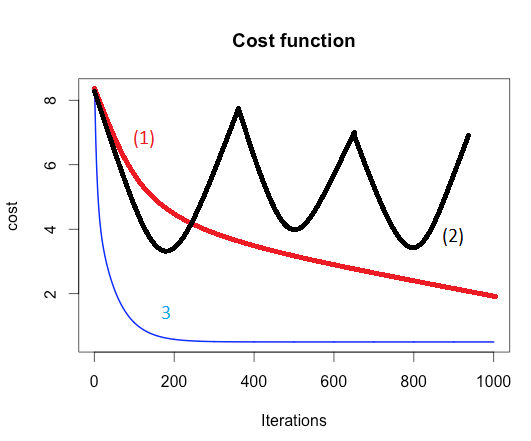
\includegraphics[totalheight=6 cm]{learningRate.png}
						\caption{
								\label{learningRate} If gradient descent works, $J(\theta)$ must decrease after each iteration (3). If $\alpha$ is too small, Gradient Descent will slowly converge (1). But if $\alpha$ too large, Gradient descent woudl not converge ((case 2) or $J(\theta)$ increases) }
\end{figure}
A good approach is to try a series of $\alpha$ values: 0.001, 0.01, 0.1, 1 and choose $\alpha$ that gives fastest converging gradient descent.
One can also try to reduce the step size as the number of iterations increases:
\begin{align}
\alpha = \frac{\alpha_0}{t}
\end{align}
where $t$ is the iteration
\subsection{Polynomial regression}

\begin{itemize}
\item Model exple 1: $\theta_0 + \theta_1 x + \theta_2 x^2 + \theta_3 x^3$ \\
How to convert it in to hypothesis: use $x_1=$size, $x_2= (\mathrm{size})^2$, $x_3= (\mathrm{size})^3$. then, $h_{\theta}(x)$ becomes:
\begin{align*}
			h_{\theta}(x) = \theta_0 + \theta_1 x_1 + \theta_2 x_2 + \theta_3 x_3
\end{align*}

\item Model exple 2: $\theta_0 + \theta_1 x + \theta_2 \sqrt(x) $\\
How to convert it in to hypothesis: use $x_1=$size, $x_2= (\mathrm{size})^0.5$, then, $h_{\theta}(x)$ becomes:
\begin{align*}
			h_{\theta}(x) = \theta_0 + \theta_1 x_1 + \theta_2 x_2
\end{align*}
\end{itemize}

\section{Normal Equations}
Normal equations provides an analytical solution to $\partial J(\theta)/ \partial \theta = 0$.
\begin{align*}
			\nabla _{\theta} J = 	\begin{bmatrix} \partial J / \partial \theta_0 \\ \partial J / \partial \theta_1\\ .\\ . \\ . \\\partial J / \partial \theta_n \end{bmatrix} \ \in \mathbb{R}^{(n+1)}
\end{align*}
Rewrite gradient descent:\\
\begin{tikzpicture}[node distance=4cm]
\node (start1) [smalldetail] {$\theta := \theta - \alpha \nabla _{\theta} J$ };
\node (dec1a) [smalldetail, below of=start1, xshift=-1.8cm, yshift=2cm] {$\in \mathbb{R}^{(n+1)}$};
\node (dec1b) [smalldetail, below of=start1, xshift=3cm, yshift=2cm] {$\in \mathbb{R}^{(n+1)}$};
\draw[-latex,line width=0.5mm] (dec1a) -- (-1.5,-0.2);
\draw[-latex,line width=0.5mm] (dec1b) -- (1,-0.2);
\end{tikzpicture}
\\
\\

Design matrix $X$ contains all the inputs from training set:
\begin{align*}
			X = \begin{bmatrix} \mathrm{--} (x^{(1)})^{\mathrm{T}} \mathrm{--} \\ \mathrm{--} (x^{(2)})^{\mathrm{T}} \mathrm{--} \\ \mathrm{--}\\ . \\ . \\ \mathrm{--} (x^{(m)})^{\mathrm{T}} \mathrm{--} \end{bmatrix} = 
			\begin{bmatrix} 
						x_0 ^{(1)} & x_1 ^{(1)} & x_2 ^{(1)} & ......& x_n ^{(1)} \\
						x_0 ^{(2)} & x_1 ^{(2)} & x_2 ^{(2)} & ......& x_n ^{(2)} \\
						. & . & . & ......&  \\
						. & . & . & ......&  \\
						. & . & . & ......&  \\
						x_0^{(m)} & x_1 ^{(m)} & x_2 ^{(m)} & ......& x_n ^{(m)} \\
			\end{bmatrix}
\end{align*}
is a ($m \times (n+1)$) matrix with $X^{(i)} = \left[\begin{smallmatrix} x_0 ^{(i)} \\ x_1 ^{(i)}\\x_2 ^{(i)}\\.\\.\\.\\x_n ^{(i)}
 \end{smallmatrix} \right]$ 
\begin{align*}
			X \times \theta = 
			\begin{bmatrix} 
						x_0 ^{(1)} & x_1 ^{(1)} & x_2 ^{(1)} & ......& x_n ^{(1)} \\
						x_0 ^{(2)} & x_1 ^{(2)} & x_2 ^{(2)} & ......& x_n ^{(2)} \\
						. & . & . & ......&  \\
						. & . & . & ......&  \\
						. & . & . & ......&  \\
						x_0^{(m)} & x_1 ^{(m)} & x_2 ^{(m)} & ......& x_n ^{(m)} \\
			\end{bmatrix} \times
			\begin{bmatrix} 
						\theta_0 \\
						\theta_1 \\
						.  \\
						.  \\
						.  \\
						\theta_n \\
			\end{bmatrix} 
			= \begin{bmatrix} 
				(x^{(1)})^{\mathrm{T}} \ \theta \\
			  (x^{(2)})^{\mathrm{T}} \ \theta \\
			  (x^{(3)})^{\mathrm{T}} \ \theta \\
			  ... \\
			  ... \\
			  ... \\
			  (x^{(m)})^{\mathrm{T}} \ \theta
			\end{bmatrix}	= 
			\begin{bmatrix} 
				h_{\theta}(x^{(1)}) \\
			  h_{\theta}(x^{(2)}) \\
			  h_{\theta}(x^{(3)}) \\
			  ... \\
			  ... \\
			  ... \\
			  h_{\theta}(x^{(m)}) \\
			\end{bmatrix}
\end{align*}

\begin{align*}
\vec{y} = \begin{bmatrix} 
				y^{(1)} \\
			  y^{(2)} \\
			  y^{(3)} \\
			  ... \\
			  ... \\
			  ... \\
			  y^{(m)} \\
			\end{bmatrix}
			\in \mathbb{R}^{(m \times 1)}
\end{align*}

and :
\begin{align*}
X \theta - \vec{y} = \begin{bmatrix} 
				h(x^{(1)}) - y^{(1)} \\
			  h(x^{(2)}) - y^{(2)} \\
			  h(x^{(3)}) - y^{(3)} \\
			  ... \\
			  ... \\
			  ... \\
			  h(x^{(m)}) - y^{(m)} \\
			\end{bmatrix}
\end{align*}
For a vector $z$, $z^{\mathrm{T}} . z = \sum z_i ^2$, hence:
\begin{align*}
\frac{1}{2} \left(X \theta - y \right)^{\mathrm{T}}\left(X \theta - y \right) = \frac{1}{2} \sum_{i=1} ^m \left(h(x^{i})-y^{i} \right)^2 = J(\theta)
\end{align*}

Minimize $J(\theta)$ for every $j$:
\begin{align*}
\begin{split}
 \nabla_{\theta} J(\theta) = 0 \\
 \nabla_{\theta}  \frac{1}{2} \left(X \theta - y \right)^{\mathrm{T}}\left(X \theta - y \right) = 0 \\
 \frac{1}{2}\nabla_{\theta} \left( \theta ^{\mathrm{T}} X^{\mathrm{T}}X \theta - y^{\mathrm{T}} X \theta - \theta^{\mathrm{T}} X ^{\mathrm{T}} y + y^{\mathrm{T}} y \right) = 0 \\
\end{split}
\end{align*}

$J(\theta) \in \mathbb{R}$ so $\mathrm{tr}(J(\theta)) = J(\theta)$ $\Rightarrow$  $\nabla _{\theta} (J(\theta)) = \nabla _{\theta} \mathrm{tr}(J(\theta))$.\\

\begin{align*}
\begin{split}
   \frac{1}{2}\nabla_{\theta} \mathrm{tr} \left( \theta^{\mathrm{T}} X^{\mathrm{T}} X \theta - \theta ^{\mathrm{T}} X^{\mathrm{T}} y - y^{\mathrm{T}} X \theta + y^{\mathrm{T}} y \right) & = 0\\
	 \frac{1}{2}\nabla_{\theta} \mathrm{tr} \left( \theta^{\mathrm{T}} X^{\mathrm{T}} X \theta \right) - \frac{1}{2}\nabla_{\theta} \mathrm{tr}\left( \theta ^{\mathrm{T}} X^{\mathrm{T}} y \right)  - \frac{1}{2}\nabla_{\theta} \mathrm{tr} \left(  y^{\mathrm{T}} X \theta \right ) + \frac{1}{2}\nabla_{\theta} \mathrm{tr} \left(  y^{\mathrm{T}} y \right) & = 0
	\end{split}
\end{align*}
$y^{\mathrm{T}}y$ does not depend on $\theta$ so $\nabla_{\theta} y^{\mathrm{T}}y = 0$:
\begin{align*}
	 \frac{1}{2}\nabla_{\theta} \mathrm{tr} \left( \theta^{\mathrm{T}} X^{\mathrm{T}} X \theta \right) - \frac{1}{2}\nabla_{\theta} \mathrm{tr}\left( \theta ^{\mathrm{T}} X^{\mathrm{T}} y \right)  - \frac{1}{2}\nabla_{\theta} \mathrm{tr} \left(  y^{\mathrm{T}} X \theta \right ) = 0
\end{align*}

Note that $\theta^{\mathrm{T}} X^{\mathrm{T}} y \in \mathbb{R}$ (If $z \in \mathbb{R}$, then $z^{\mathrm{T}} = z$), so: $(\theta^{\mathrm{T}} X^{\mathrm{T}} y)^{\mathrm{T}}= y^{\mathrm{T}} X \theta$ 

\begin{align*}
	 \frac{1}{2}\nabla_{\theta} \mathrm{tr} \left( \theta^{\mathrm{T}} X^{\mathrm{T}} X \theta \right) - \nabla_{\theta} \mathrm{tr} \left(  y^{\mathrm{T}} X \theta \right ) = 0
\end{align*}

By the property of permutation: $\theta^{\mathrm{T}} X^{\mathrm{T}} X \theta =  \theta \theta^{\mathrm{T}} X^{\mathrm{T}} X $, and: 
\begin{align*}
\nabla_{\theta} \mathrm{tr}(\theta \theta^{\mathrm{T}} X^{\mathrm{T}} X)
= \nabla_{\theta} \mathrm{tr} (\underbrace{\theta}_{A}  \underbrace{I}_{B} \underbrace{\theta^{\mathrm{T}}}_{A^{\mathrm{T}}} \underbrace{X^{\mathrm{T}} X}_{C})
= \underbrace{X^{\mathrm{T}}X}_{C} \underbrace{\theta}_{A} \underbrace{I}_{B} + \underbrace{X^{\mathrm{T}}X}_{C^{\mathrm{T}}} \underbrace{\theta}_{A} \underbrace{I}_{B^{\mathrm{T}}}
\end{align*}


\begin{align*}
\nabla _{\theta} \mathrm{tr} \underbrace{y^{\mathrm{T}} X}_{B} \underbrace{\theta}_{A} = \underbrace{X^{\mathrm{T}} y}_{B^{\mathrm{T}}}  
\end{align*}

Hence:
\begin{align*}
\nabla_{\theta} J(\theta) = \frac{1}{2} \left(X^{\mathrm{T}} X \theta + X^{\mathrm{T}} X \theta\ right) - X^{\mathrm{T}} y \right) = 0 
\end{align*}

Finally:
\begin{align*}
X^{\mathrm{T}} X \theta  = X^{\mathrm{T}} y = 0 \\
\theta = \left(X^{\mathrm{T}} X\right)^{-1} X^{\mathrm{T}} y
\end{align*}

Pros and Cons of Gradient Descent and Normal Equations: \\
\begin{tabular}{ | p{5cm} || p{5cm} |  }
\hline
 Gradient Descent & Normal Equations \\
 \hline
 Need to choose $\alpha$ & No need to choose $\alpha$ \\
 Need to use many iterations & No iteration \\
 works well even with large Nbrs of features & slow for very large nbrs of features \\
 & Need to compute $(XX^{\mathrm{T}})^{-1}$ : cost of inverting matrix is O($n^3$) for a $n \times n$ matrix\\
\end{tabular}

 
\begin{appendices}
\chapter{Linear Algebra Review}
\section{1-indexed versus 0-indexed vector matrix}

\begin{align*}
		Y(\mathrm{1-indexed}) = \begin{bmatrix} y_1 \\ y_2 \\ y_3 \end{bmatrix}  \mathrm{and}  Y(\mathrm{0-indexed}) = \begin{bmatrix} y_0 \\ y_1 \\ y_2 \end{bmatrix},
\end{align*}
\\

\section{Matrix}
\subsection {Matrix size}
\begin{align*}
		A = \begin{bmatrix} a & b & c \\ d & e & f \\ g & h & i \\ j & k & l \end{bmatrix},
\end{align*}
is a 4(rows) $\times$ 3(cols) matrix ($\mathbb{R} ^ {3 \times 2}$ matrix). Length = \# Rows $\times$ \#Cols
\\
$A_{ij}$ corresponds to value at row $i^{\mathrm{th}}$ and col $j^{\mathrm{th}}$
\\
\begin{align*}
		 A = \begin{bmatrix} a \\ d \\ g \\ j 
		\end{bmatrix},
\end{align*}
is a \textbf{vector} matrix ($n \times 1$)

\subsection {Matrix Operation}
\subsubsection{Matrix addition}
 \begin{align*}
		A + B = \begin{bmatrix} a & b \\ c & d \end{bmatrix} + \begin{bmatrix} w & x \\ y & z\end{bmatrix} = \begin{bmatrix} (a+w) & (b+x) \\ (c+y) & (d+z)\end{bmatrix},
\end{align*}
\subsubsection{Matrix scalar multiplication}
\begin{align*}
	 A \times x = x \times A = x \times \begin{bmatrix} a & b \\ c & d \end{bmatrix} = \begin{bmatrix} (a\times x) & (b \times x) \\ (c \times x) & (d \times x)\end{bmatrix},
\end{align*}
\subsubsection{Multiplication of 2 matrix}
$ A \times B$ requires that the \# of rows of $A$ be equal to \# of cols of B. \\
Matrix $\times$ a vector = a vector ($n\times m$) matrix $\times$ ($m\times 1$) vector = $n \times 1$ vector
\begin{align*}
		A \times B = \begin{bmatrix} a & b \\ c & d \\ e & f \end{bmatrix} \times  \begin{bmatrix} x \\ y \end{bmatrix}= \begin{bmatrix} (ax + by) \\ (cx+dy) \\ (ex+fy)\end{bmatrix}
\end{align*}		
\\ 
Matrix multiplication  properties:
\begin{itemize}
\item Not commutative: $A \times B \neq B \times A$
\item associative : $A \times B \times C = (A \times B)\times C = A \times(B \times C)$
\end{itemize}
\subsubsection{Matrix Identity}
$A \times I = A$, where I is a matrix identity:
\begin{align*}
		I = \begin{bmatrix} 1 & 0 &0 & 0\\ 0 & 1 &0 & 0\\ 0 & 0 &1 & 0\\ 0 & 0 &0 &1  \end{bmatrix}
\end{align*}
\subsubsection{Matrix Inverse}
Inverse of $A$ is denoted $A^{-1}$, and : 
\begin{align*}
		A \times A^{-1} = I
\end{align*}
A non-square matrix does not have an inverse.

\subsubsection{Transpose matrix $A^{\mathrm{T}}$}
\begin{align*}
		A = \begin{bmatrix} a & b \\ c & d \\ e & f  \end{bmatrix}
\end{align*}
\begin{align*}
		A^{\mathrm{T}} = \begin{bmatrix} a & c & e \\ b & d & f  \end{bmatrix}
\end{align*}
so $A_{ij} = A_{ji} ^{T}$

\subsection{Derivative $\nabla_A f(A)$}
For a function $f$: $\mathbb{R} ^ {(m \times n)} \rightarrow  \mathbb{R}$ mapping from $m$-by-$n$ matrix to the real numbers, we define the derivative of $f$ with respect to $A$ to be:
\begin{align*}
		\nabla_A f(A) = \begin{bmatrix} \partial f/ \partial A_{11} & \partial f/ \partial A_{12} & ......&\partial f/ \partial A_{1n} \\
		                                 .. & .. & .. & .. \\
																		 .. & .. & .. & .. \\
																		 .. & .. & .. & .. \\
		                                \partial f/ \partial A_{m1} & \partial f/ \partial A_{m2} & ......&\partial f/ \partial A_{mn} \\
		\end{bmatrix}
\end{align*}
so $\nabla_A f(A)$ is itself a $\mathbb{R}^{(m \times n)}$ whose $(i,j)$ elements is $\partial f / \partial A_{ij}$. \\
\\
For example: $A = \left[ \begin{smallmatrix} A_{11} & A_{12}\\ A_{21} & A_{22} \\ \end{smallmatrix} \right]$ is a $2\times2$ matrix, and $f: \mathbb{R}^{(2 \times 2)} \rightarrow \mathbb{R} $ is: $f(A)= \frac{3}{2} A_{11} + 5A_{12}^2 + A_{21}A_{22}$. Then $\nabla_A f(A) = \left[ \begin{smallmatrix} 3/2 & 10 A_{12}\\ A_{22} & A_{21} \\ \end{smallmatrix} \right]$

\subsection{Trace}
\begin{align*}
		\mathrm{tr} A = \sum_{i=1} ^n A_{ii} \mathrm{  \ if A} \in \mathbb{R}^{n \times n}
\end{align*}
\begin{align*}
		\mathrm{tr} (A \times B) = \mathrm{tr} (B \times A) 
\end{align*}
\begin{align*}
		\mathrm{tr} (A B C) = \mathrm{tr} (C A B) = \mathrm{tr} (B C A)
\end{align*}
\begin{align*}
		\mathrm{tr} (A B C D) = \mathrm{tr} (D A B C) = \mathrm{tr} ( C D A B )
\end{align*}

If $A$ and $B$ are square matrix:
\begin{align*}
		\mathrm{tr} A = \mathrm{tr} A^{\mathrm{T}}
\end{align*}
\begin{align*}
		\mathrm{tr} (A+B) = \mathrm{tr} A + \mathrm{tr} B
\end{align*}

If $a \in \mathbb{R}$:
\begin{align*}
		\mathrm{tr} (a) = a
\end{align*}

If $f(A) = \mathrm{tr}(AB)$
\begin{align*}
		\nabla_A \mathrm{tr} (A B) = B^{\mathrm{T}}
\end{align*}
\begin{align*}
		\nabla_A \mathrm{tr} (A BA^{\mathrm{T}}C) = CAB + C^{\mathrm{T}}AB^{\mathrm{T}}
\end{align*}

\chapter{Matlab}
\begin{itemize}
\item disp(a) /*show the matrix
\item a=3.14567 \\
disp(sprintf('2 decimals: \%0.2f', a))

\item define $a$ row vector: v=[1 2 3]  $\rightarrow$ v[1,2,3]

\item define $a$ col vector: v=[1; 2; 3]  $\rightarrow$ $a = \left[ \begin{smallmatrix} 1 \\ 2 \\ 3 \end{smallmatrix} \right]$

\item define $a$ matrix (3$\times$2): a=[1 2; 3 4; 5 6] $\rightarrow$ $a = \left[ \begin{smallmatrix} 1 & 2\\ 3 & 4 \\ 5 & 6 \end{smallmatrix} \right]$

\item eye(2) gives a 2$\times$2 Identity matrix $\rightarrow$ $a = \left[ \begin{smallmatrix} 1 & 0 \\ 0 & 1  \end{smallmatrix} \right]$

\item zeros(2) gives a 2$\times$2 matrix with only elements 0 $\rightarrow$ $a = \left[ \begin{smallmatrix} 0 & 0 \\ 0 & 0  \end{smallmatrix} \right]$

\item ones(2) gives a 2$\times$2 matrix with only elements 1 $\rightarrow$ $a = \left[ \begin{smallmatrix} 1 & 1 \\ 1 & 1  \end{smallmatrix} \right]$

\item $a$ matrix (3$\times$2): a=[1 2; 3 4; 5 6] $\rightarrow$ $a = \left[ \begin{smallmatrix} 1 & 2\\ 3 & 4 \\ 5 & 6 \end{smallmatrix} \right]$ \\
sz = size(A) $\rightarrow$ [3,2] \\
size(A,1) $\rightarrow$ nbrs of rows (3) \\
size(A,2) $\rightarrow$ nbrs of cos (2) \\
For a vector $A$ use length($A$)

\item pwd $\rightarrow$ current directory
\item load(filename)
\item who $\rightarrow$ show what variables are in memory
\item whos $\rightarrow$ show list of variables (with size, type) in memory
\item clear $\rightarrow$ remove all variables from memory
\item save hello.txt $v$ -ascii $\rightarrow$ save $v$ as ascii
\item save hello.m $v$  $\rightarrow$ save $v$ as matlab file

\item  Elements of $A = \left[ \begin{smallmatrix} 1 & 2\\ 3 & 4 \\ 5 & 6 \end{smallmatrix} \right]$ \\
$A$(3,2) $\rightarrow$ 6 \\
$A$(2, :) $\rightarrow$ return row \# 2 : (3 4) \\
$A$(:, 2) $\rightarrow$ return col \# 2 : $\left[ \begin{smallmatrix} 2\\ 4 \\ 6 \end{smallmatrix} \right]$ \\

\item  pinv(A) $\rightarrow$ $A^{-1}$

\item $A = \left[ \begin{smallmatrix} 1 & 2\\ 3 & 4 \\ 5 & 6 \end{smallmatrix} \right]$ and $B = \left[ \begin{smallmatrix} 11 & 12\\ 13 & 14 \\ 15 & 16 \end{smallmatrix} \right]$ \\
$A.*B$ $\rightarrow$ $\left[ \begin{smallmatrix} 11 & 24\\ 39 & 56 \\ 75 & 96 \end{smallmatrix} \right]$ \\
(.*) element-wise multiplication of 2 matrix
\end{itemize}

\chapter{Exercise: Gradient Descent Matlab}
\begin{python}
data = load( 'data.txt' );
X = data( : , 1:2 );
y = data( : , 3 );
m = length( y );
# scale features
mu = zeros( 1, size( X, 2 ) );
sigma = zeros( 1, size( X, 2 ) );
X_norm = X;

mu = mu * mean( X )
sigma = sigma * std( X )

X_norm = ( X - mu ) ./sigma;
X_norm = [ ones( m, 1 ), X_norm ]  #add intercept term to X

# Gradient descent
alpha = 0.01;
num_iters = 400;

# Initialize theta and J
theta = zeros( 3, 1);
J = 0;
J_history = zeros( num_iters, 1);

for iter = 1:num_iters
	theta = theta - alpha/m * X' * ( X * theta - y );
  # Compute Cost'
	prediction = X * theta;
	sqErr = ( prediction - y ).^2 ;
	J = 1/(2 * m) sum( sqErr );
	J_history ( iter ) = J;

plot( J_history );
xlabel( 'Nb of iterations' );
ylabel( 'Cost J' );
\end{python}


\end{appendices}

\end{document}